\documentclass[slidestop]{beamer}
\usepackage{beamerthemesplit}
\usepackage{graphics}
\usepackage{pstricks}

\graphicspath{{./}}

\title{The Libre-SOC OpenPOWER 180nm ASIC}
\author{Luke Kenneth Casson Leighton}

\begin{document}

\frame{
   \begin{center}
    \huge{Libre-SOC Power ISA 180nm ASIC}\\
    \vspace{32pt}
    \Large{Concept to completion:}\\
    \Large{Why we chose nmigen and OpenPOWER}\\
    \Large{What happened along the way}\\
    \vspace{24pt}
    \Large{IIT Roorkee 2021}\\
    \vspace{16pt}
    \large{Sponsored by NLnet's PET Programme}\\
    \vspace{6pt}
    \large{\today}
  \end{center}
}


\frame{\frametitle{Why start a new SoC?}

 \begin{itemize}
   \item Intel Management Engine, Apple QA issues, Spectre\vspace{6pt}
   \item Zero transparency: commodity hardware cannot be audited.
         \vspace{6pt}
   \item Endless proprietary drivers, "simplest" solution: \\
         License proprietary hard macros (with proprietary firmware)\\
   		 Adversely affects product development cost\\
   		due to opaque driver bugs (Samsung S3C6410 / S5P100)
   		 \vspace{6pt}
   \item Alternative: Intel and Valve-Steam collaboration\\
         "Most productive business meeting ever!"\\
         https://tinyurl.com/valve-steam-intel
		\vspace{6pt}
   \item Ultimately it is a strategic \textit{business} objective to
         develop entirely Libre hardware, firmware and drivers.
  \end{itemize}
}


\frame{\frametitle{Why OpenPOWER?}

\vspace{15pt}

 \begin{itemize}
   \item Good ecosystem essential\\
   		 linux kernel, u-boot, compilers, OSes,\\
   		 Reference Implementation(s)\vspace{10pt}
   \item Supportive Foundation and Members\\
   		 need to be able to submit ISA augmentations\\
   		 (for proper peer review)\vspace{10pt}
   \item No NDAs, full transparency must be acceptable\\
	     due to being funded under NLnet's PET Programme\vspace{10pt}
   \item OpenPOWER: established for decades, excellent Foundation,\\
   	     Microwatt as Reference, approachable and friendly.
  \end{itemize}
}


\frame{\frametitle{Choosing an HDL}

 \begin{itemize}
   \item 3 months careful evaluation: Chisel3, MyHDL, Verilog, VHDL, migen,
   		nmigen
   \item Love the OO capabilities of Chisel3, shame about the TIOBE Index
   		(below 20th)
   	\item MyHDL is in python, but limits to a subset of python.  Also,
   		 community not as large as for nmigen.
   \item migen extremely inconvenient: errors created and not caught until
         ASIC synthesis level!
    \item Verilog is 1980s (like BASIC and FORTRAN) - considered "machine
         code"
    \item VHDL is great (has records) but still no OO capability
    \item Ultimately nmigen chosen due to large community, and because
         python is 3rd on the TIOBE index (contd)
  \end{itemize}
}

\frame{\frametitle{Why nmigen?}

 \begin{itemize}
   \item Uses python to build an AST (Abstract Syntax Tree).
         Actually hands that over to yosys (to create ILANG file)
         after which verilog can (if necessary) be created
   \item Deterministic synthesiseable behaviour (Signals are declared
         with their reset pattern: no more forgetting "if rst" block).
   \item python OO programming techniques can be deployed.  classes
         and functions created which pass in parameters which change
         what HDL is created (IEEE754 FP16 / 32 / 64 for example)
   \item python-based for-loops can e.g. read CSV files then generate
         a hierarchical nested suite of HDL Switch / Case statements
         (this is how the Libre-soc PowerISA decoder is implemented)
   \item extreme OO abstraction can even be used to create "dynamic
         partitioned Signals" that have the same operator-overloaded
         "add", "subtract", "greater-than" operators
   
  \end{itemize}
}


\frame{\frametitle{Software Engineering Techniques}

 \begin{itemize}
   \item Entire project run along standard Libre Software Project
        Management: public bugtracker, public mailing lists, public IRC,
        public git repositories, Charter http://libre-soc.org/charter/
   \item None of our engineers are Hardware trained! They are all
         software developers who learned HDL!
   \item The other way round makes life much harder.
   \item Like Microwatt, we develop unit tests, use git revision control,
   		and bugtrackers (TODO, still - set up Continuous Integration)
   \item Unlike Microwatt, we also have a wiki for all documentation
         (backed by a git repository with full revision control)
   \item Software Engineering techniques are critical for large project
   		management! unit tests, unit tests, unit tests...
  \end{itemize}
}

\frame{\frametitle{Auditability and Transparency}

 \begin{itemize}
   \item Funded by NLnet's "Privacy and Enhanced Trust Programme"
   \item Matches well with business objectives to provide customers
   		 with ability to inspect down to Gate Level (GDS-II files)
   \item (Impossible for Intel etc to do, due to 3rd party licensing
   		of 50-60 pieces of HDL).
   	\item Sorbonne University LIP6.fr http://coriolis2.lip6.fr is
   	     an entirely Libre-licensed VLSI toolchain
   	\item (coriolis2 is "Zero config" from HDL to GDS-II)
   	\item Chips4Makers.io Cell Library - FlexLib - has "Symbolic"
   	      and "Real" versions.
   	Symbolic is public and published, uses FreePDK45
   	"Real" is NDA'd with Foundry.
    \item Therefore: Libre-SOC team can work side-by-side with
          LIP6.fr WITHOUT signing a Foundry NDA.
          
  \end{itemize}
}

\frame{\frametitle{Development Process}

 \begin{itemize}
   \item nmigen HDL, in python, converted to verilog using yosys
   \item developed several thousand unit tests at every level
   \item Jean-Paul Chaput improved coriolis2 to cope with automated layout
   		of 130,000 Cells. Antenna, buffers, etc.
   	\item Chips4Makers FlexLib Cell Library also needed development, including
   	   a custom 4k SRAM block (under NDA, sorry)
   	\item Professor Galayko developed a Voltage-Controlled PLL, capable of
   		between 150 and 900 mhz.
    \item Marie-Minerve Louerat developed and ran HITAS (Static Timing 
    Analysis tool).
    \item Tried simulating the laid-out ASIC, required too much resources.
        Instead, simulated smaller ASICs
   
  \end{itemize}
}

\frame{\frametitle{ASIC diagram sent to TSMC}

\begin{center}
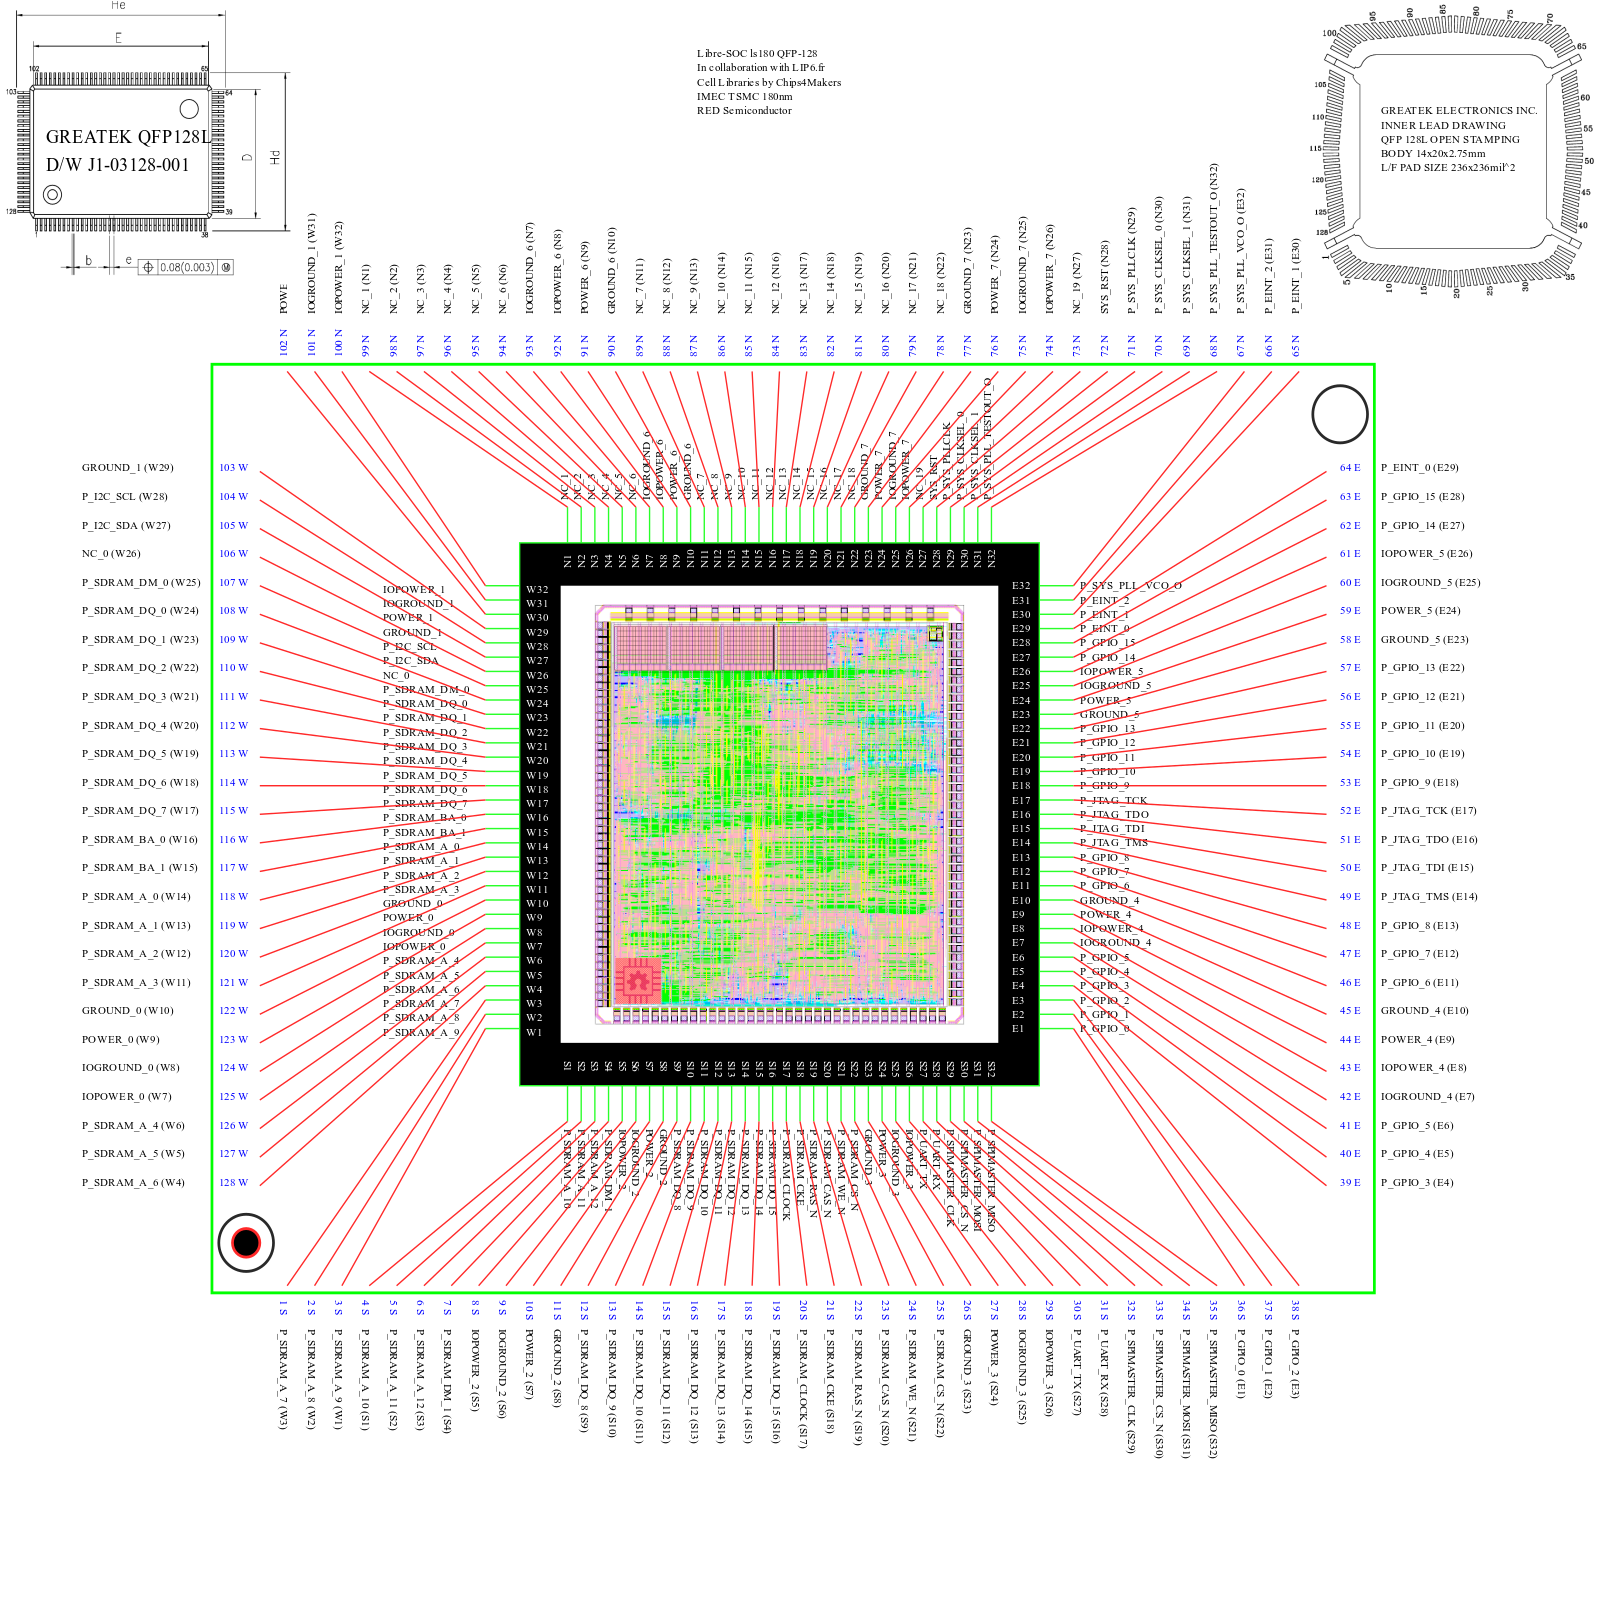
\includegraphics[width=0.7\textwidth]{ls180.png}
\end{center}

}



\frame{
  \begin{center}
    {\Huge The end\vspace{12pt}\\
		   Thank you\vspace{12pt}\\
		   Questions?\vspace{12pt}
	}
  \end{center}
  
  \begin{itemize}
	\item Discussion: http://lists.libre-soc.org
	\item Libera IRC \#libre-soc
	\item http://libre-soc.org/
	\item http://nlnet.nl/PET
	\item https://libre-soc.org/nlnet/\#faq
  \end{itemize}
}


\end{document}
